\chapter{Fundamentação Teórica}
Este capítulo busca contextualizar os principais conceitos abordados no presente trabalho, tais como os materiais utilizados como base e também a tecnologia adotada no desenvolvimento do projeto. Ao final, são listados e discutidos alguns trabalhos correlatos.

\section{Estratégia Nacional de Educação Financeira}

A \cite{ENEF} representa uma resposta proativa e estruturada às crescentes demandas de uma sociedade que enfrenta desafios financeiros complexos. Instituída visando aprimorar a conscientização financeira da população brasileira, a ENEF busca não apenas promover a cidadania, mas também equipar os indivíduos com as ferramentas necessárias para tomar decisões financeiras informadas.

Essa estratégia abrange um amplo espectro de áreas de estudo, que vão desde os direitos e deveres básicos até tópicos mais complexos, como investimentos, previdência e planejamento financeiro. A inclusão de temas como poupança, crédito, seguros e consumo demonstra a abordagem abrangente adotada pela \cite{ENEF}. Ao abordar temas tão variados, ela reconhece e enfatiza que a educação financeira é um processo contínuo, que deve começar na infância e continuar ao longo da vida.

A \cite{ENEF} destaca-se por sua abordagem prática, evidenciada por sua ampla variedade de materiais didáticos. Foram elaborados 24 livros especificamente alinhados com sua missão educacional. Cada livro foi cuidadosamente desenvolvido para atender às necessidades de diferentes faixas etárias: 18 destinados ao Ensino Fundamental e os 6 restantes focados no Ensino Médio. Uma característica notável é a separação dos livros em materiais específicos para alunos e guias para professores, garantindo que o conteúdo seja adequadamente direcionado para cada público.

Os primeiros livros pretendem familiarizar os alunos do Ensino Fundamental com conceitos fundamentais de cidadania \cite{ENEF_EF}. Por meio de situações cotidianas, como a organização de uma sala de aula ou a coordenação de eventos escolares, os alunos são introduzidos a princípios de planejamento e organização. Conforme avançam na série, são gradualmente expostos a temas financeiros mais sofisticados, desde o entendimento básico das contas domésticas até a compreensão da origem e da trajetória do dinheiro na sociedade.

Dentre os materiais didáticos, os chamados ``livros-jogo'' se destacam por suas narrativas envolventes. Ao invés de simplesmente transmitir informações, esses livros contam histórias que permitem aos alunos explorar cenários financeiros e entender as consequências de várias decisões. Esse enfoque narrativo é enriquecido por discussões em livros subsequentes, que oferecem \textit{insights} sobre o papel de diferentes instituições financeiras e seu impacto na sociedade.

Nos livros 5~\cite{Livro_ENEF_5_Ano} e 6~\cite{Livro_ENEF_6_Ano} da série ENEF, observa-se uma abordagem pedagógica inovadora e envolvente, que reflete a excelência e o comprometimento em proporcionar uma educação financeira de qualidade. Estes volumes adotam um formato interativo de livro-jogo. Enquanto o jogo digital foca na jogabilidade, o livro-jogo se destaca por sua capacidade de envolver o leitor em uma narrativa rica, permitindo-lhe tomar decisões que influenciam os rumos da história.

A Figura~\ref{fig:figure-1} ilustra um esquema que destaca alguns dos caminhos possíveis que a história pode seguir. Esse diagrama demonstra a complexidade e a diversidade de trajetórias que um jogador pode experimentar, refletindo diferentes escolhas financeiras e suas respectivas consequências.

\begin{figure}[ht]
	\centering
	\caption{Esquema com alguns dos caminhos possíveis da primeiro jogo/história.}
	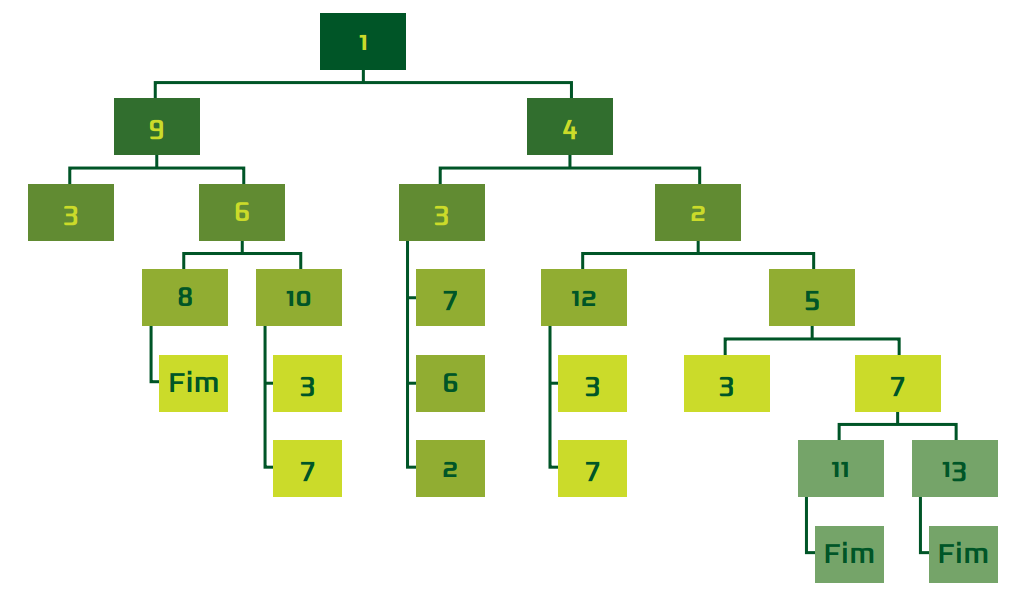
\includegraphics[scale=0.25]{Textuais/Pictures/Picture1.png}
	\fonte{\cite{Livro_ENEF_5_Ano_professor}}\label{fig:figure-1}
\end{figure}

As Figuras~\ref{fig:figure-2} e~\ref{fig:figure-3} retratam momentos cruciais na narrativa do livro-jogo. Em cada figura, o leitor é introduzido a um cenário e, posteriormente, confrontado com duas ou três opções de ação. Cada escolha desencadeia diferentes desenvolvimentos na história, ilustrando as implicações de suas decisões no mundo financeiro.

\begin{figure}[ht]
	\centering
	\caption{Momento de decisão com duas possibilidades de caminhos.}
	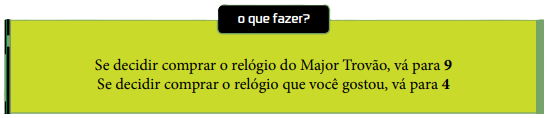
\includegraphics[scale=0.75]{Textuais/Pictures/Picture2.png}
	\fonte{\cite{Livro_ENEF_5_Ano}}\label{fig:figure-2}
\end{figure}

\begin{figure}[ht]
	\centering
	\caption{Momento de decisão com duas possibilidades de caminhos.}
	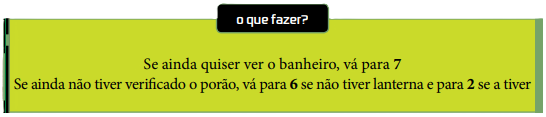
\includegraphics[scale=0.75]{Textuais/Pictures/Picture3.png}
	\fonte{\cite{Livro_ENEF_5_Ano}}\label{fig:figure-3}
\end{figure}

Na continuação da série, principalmente nas fases finais do Ensino Fundamental, a ENEF aprofunda a abordagem, introduzindo conceitos mais avançados e específicos sobre o universo financeiro \cite{ENEF_EM}. Os alunos são expostos a uma variedade de instituições financeiras e suas respectivas funções. Por exemplo, ao aprender sobre bancos, os estudantes ganham experiência sobre operações bancárias, sistemas de crédito e a importância da gestão financeira. Quando o tema é agências de viagens ou hotéis, os alunos são introduzidos ao mundo das transações comerciais, tarifas, reservas e a economia do turismo. Essa abordagem detalhada serve para ampliar o horizonte dos alunos e prepará-los para interações financeiras mais complexas no futuro.

\section{RPG Maker MZ}

O RPG Maker MZ~\cite{RPGMakerMZ} é uma plataforma de desenvolvimento de jogos notavelmente sofisticada, direcionada especificamente para a criação de Role-Playing Games (RPGs). Esta ferramenta, ilustrada na Figura~\ref{fig:rpgmaker-interface}, é equipada com uma interface de usuário intuitiva e um conjunto de recursos predefinidos. Sua concepção tem como objetivo democratizar o processo de desenvolvimento de jogos, fornecendo aos indivíduos, independentemente de seu nível de expertise no design de jogos, os meios necessários para transformar conceitos criativos em realidades interativas.

Inserida neste contexto, a capacidade do RPG Maker MZ de permitir a edição avançada de mapas e a programação de eventos condicionados pela localização geográfica no jogo destaca-se como uma de suas características mais proeminentes. O editor de mapas habilita os usuários a comporem cenários digitais minuciosamente detalhados, que vão desde extensas topografias naturais até ambientes internos complexos. A implementação de eventos baseados em localização é fundamental, atuando como um pilar para a narrativa e as mecânicas lúdicas. Desta maneira, o RPG Maker MZ estabelece um ambiente sinérgico de edição de mapas e administração de eventos, promovendo uma interação harmoniosa entre a estrutura espacial do jogo e sua trama, culminando em uma experiência de jogo coesa, imersiva e cativante~\cite{RPGMakerMZ}.

\begin{figure}[ht]
	\centering
	\caption{Interface do RPG Maker MZ~\cite{RPGMakerMZ}.}
	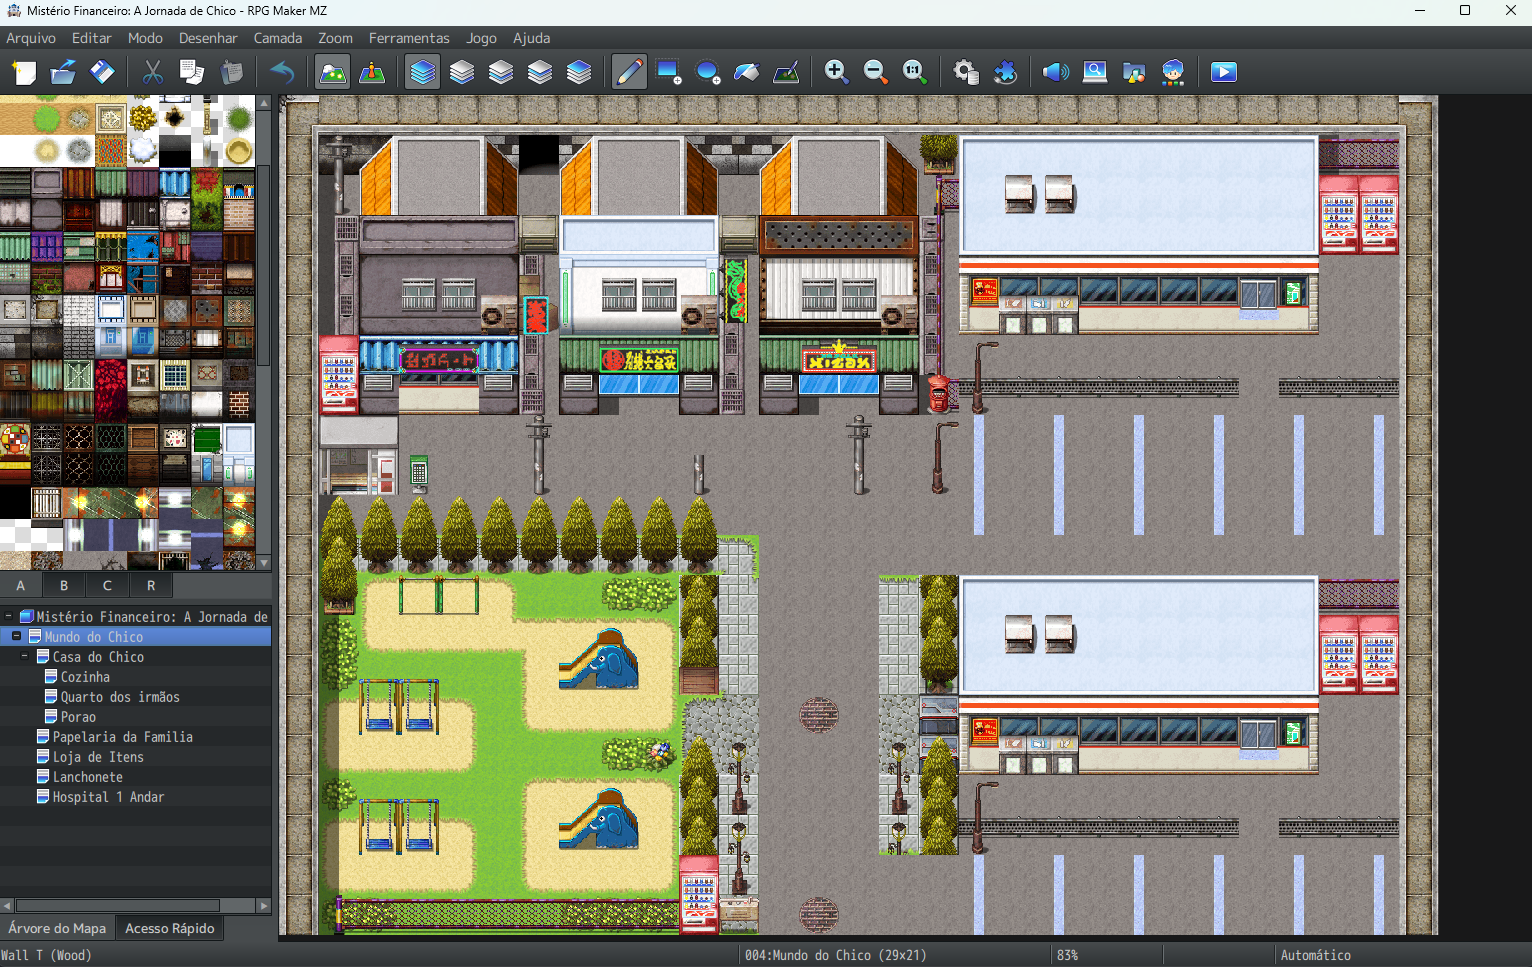
\includegraphics[scale=0.25]{Textuais/Pictures/RPGMaker_Interface.png}
	\fonte{Captura de tela do autor (2023).}\label{fig:rpgmaker-interface}
\end{figure}

\newpage

\subsubsection*{Comandos de evento}
A Figura~\ref{fig:rpgmaker-event-commands} ilustra a interface de usuário do RPG Maker MZ dedicada à configuração dos comandos de evento. Estes comandos são elementos vitais no desenvolvimento de jogos, permitindo a criação de interações narrativas, mecânicas de jogo e controle ambiental. Entre os comandos disponíveis, destacam-se aqueles frequentemente empregados pelos desenvolvedores devido à sua versatilidade e impacto significativo na jogabilidade:

\begin{itemize}
	\item \textit{\textbf{Show Text}}: Exibe texto na tela, com opções de personalização da apresentação.
	\item \textit{\textbf{Show Choices}}: Apresenta escolhas para o jogador, afetando o rumo do jogo.
	\item \textit{\textbf{Control Switches}}: Manipula interruptores que controlam eventos e condições no jogo.
	\item \textit{\textbf{Control Variables}}: Gerencia variáveis para dinâmicas complexas de jogo.
	\item \textit{\textbf{Common Event}}: Controla a chamada de outros eventos, como eventos de cenas do jogo.
	\item \textit{\textbf{Change Gold}}: Altera a quantidade de moeda do jogador, afetando possíveis transações e eventos.
	\item \textit{\textbf{Transfer Player}}: Move o jogador para diferentes localizações dentro do jogo.
	\item \textit{\textbf{Set Movement Route}}: Define rotas específicas para o movimento de personagens ou eventos.
	\item \textit{\textbf{Show Picture}}: Exibe imagens na tela para reforçar narrativas ou ilustrar itens e personagens.
	\item \textit{\textbf{Erase Picture}}: Remove imagens da tela, geralmente utilizada para limpar a interface.
	\item \textit{\textbf{Fadeout Screen}}: Realiza um efeito de transição ao escurecer a tela gradualmente.
	\item \textit{\textbf{Fadein Screen}}: Transição inversa do Fadeout, clareando a tela para o retorno à cena.
	\item \textit{\textbf{Play BGM}}: Inicia a reprodução de música de fundo para ambientação.
	\item \textit{\textbf{Game Over}}: Finaliza o jogo, mostrando a tela de fim de jogo.
	\item \textit{\textbf{Open Menu Screen}}: Abre o menu do jogo para acesso às opções e itens.
	\item \textit{\textbf{Plugin Command}}: Executa comandos de plugins, expandindo as funcionalidades do software.
\end{itemize}

\begin{figure}[ht]
	\centering
	\caption{Comandos de evento disponíveis no RPG Maker MZ~\cite{RPGMakerMZ}.}
	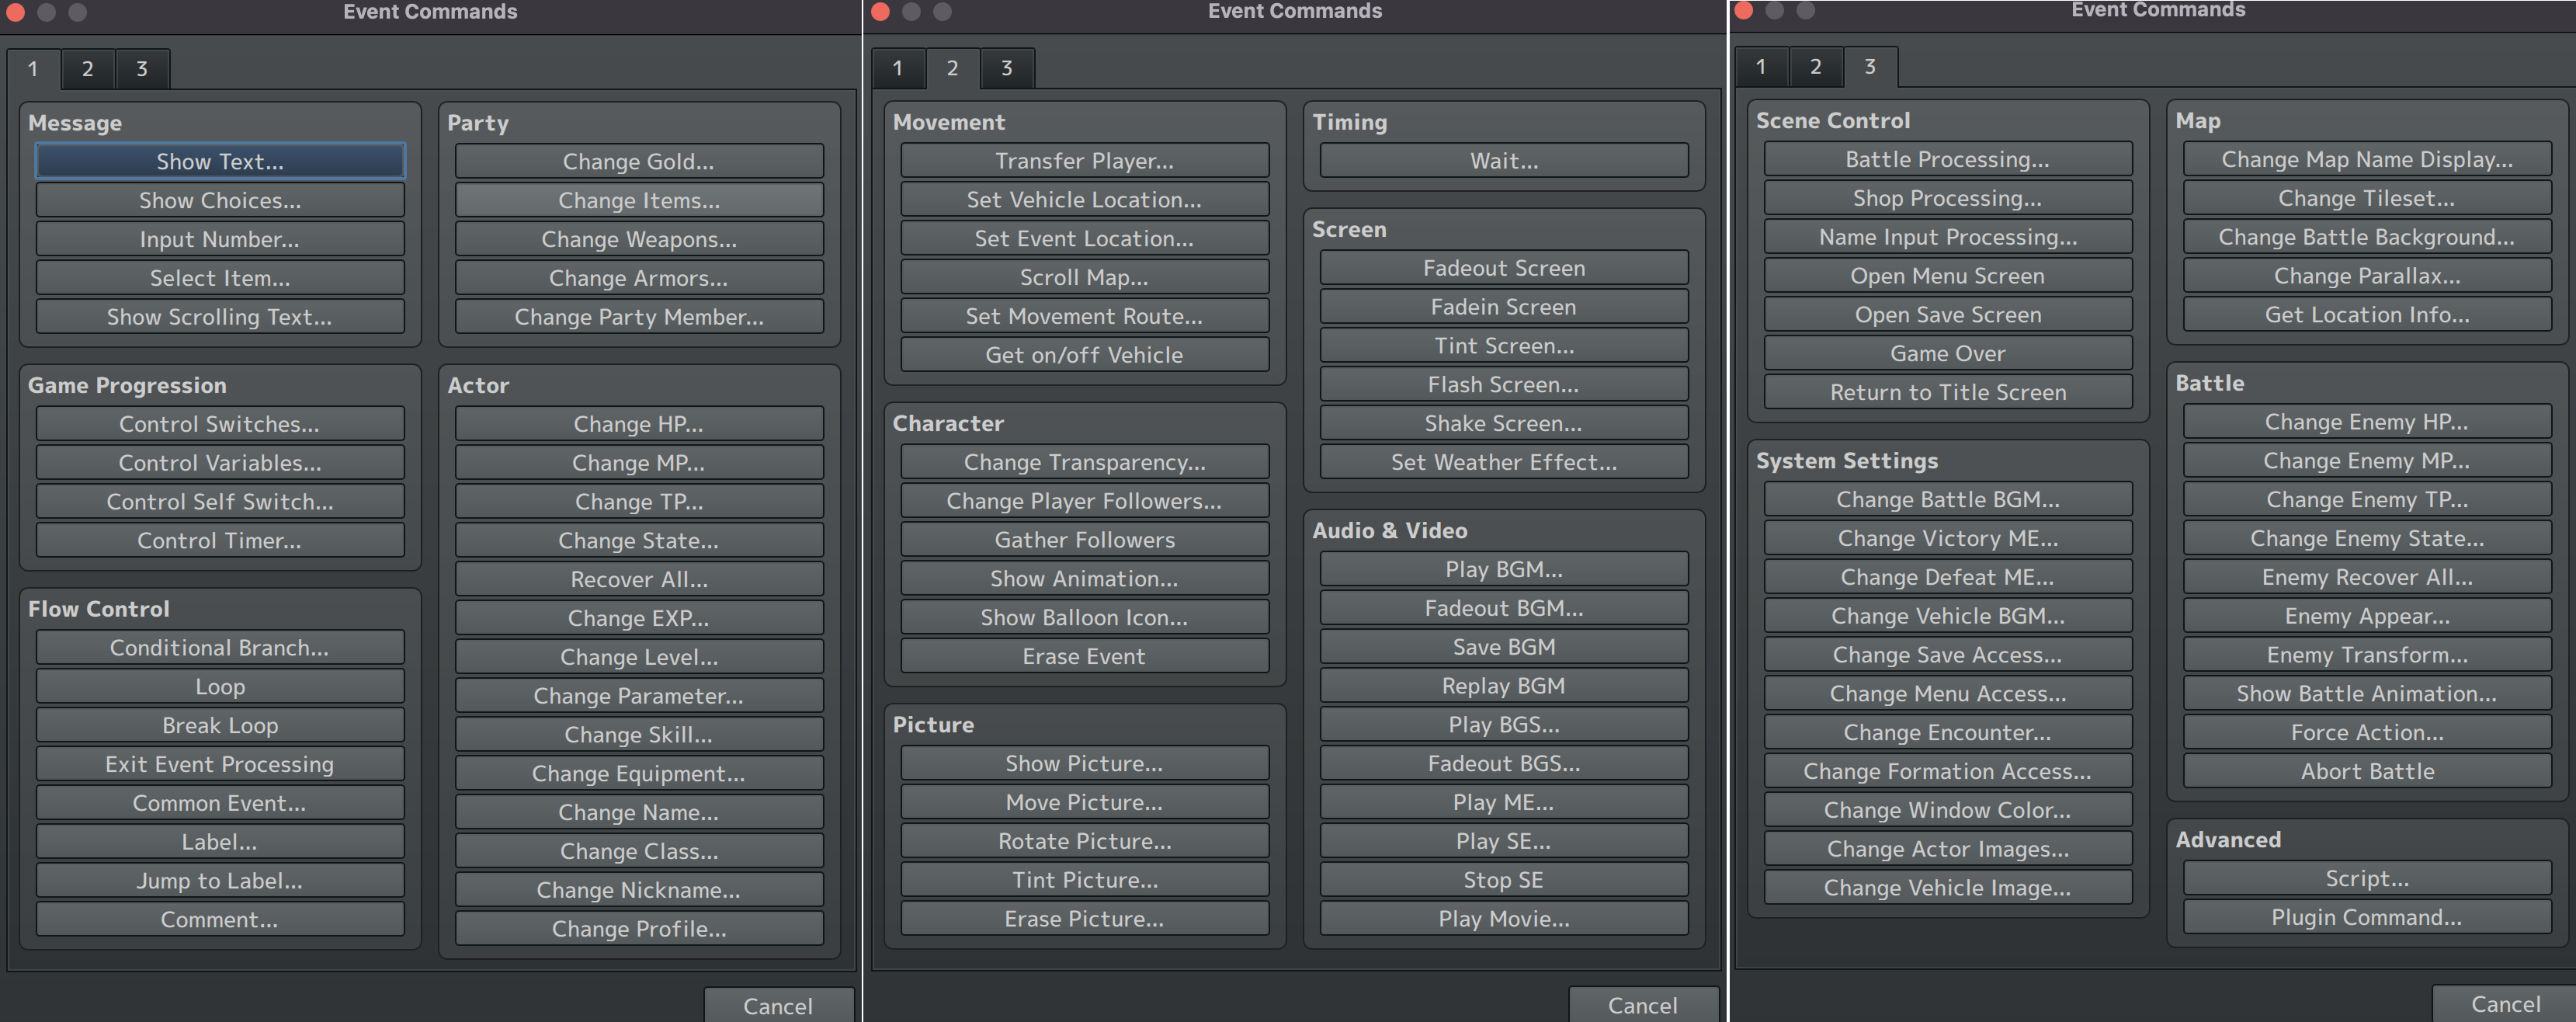
\includegraphics[scale=0.25]{Textuais/Pictures/Event-commands.png}
	\fonte{Captura de tela do autor (2023).}\label{fig:rpgmaker-event-commands}
\end{figure}

\newpage

\subsubsection*{Criador de Personagens}
O RPG Maker MZ~\cite{RPGMakerMZ} contém um módulo dedicado à criação de personagens, demonstrado na Figura~\ref{fig:rpgmaker-criador-personagens}. Esta funcionalidade permite aos usuários compor personagens personalizados através da seleção de atributos distintos como faces, penteados, expressões faciais, vestuário e acessórios. Esta variedade de opções habilita uma personalização detalhada, facilitando a criação de personagens únicos que se alinham com a narrativa e o estilo artístico do jogo.

A interface do criador de personagens, apresentada na Figura~\ref{fig:rpgmaker-criador-personagens}, é projetada para ser intuitiva, guiando os desenvolvedores na configuração dos elementos visuais dos avatares passo a passo. Tal processo não somente estabelece a identidade visual dos personagens, mas também pode influenciar suas interações e papéis dentro da dinâmica do jogo.

\begin{figure}[ht!]
	\centering
	\caption{Interface do criador de personagens no RPG Maker MZ~\cite{RPGMakerMZ}.}
	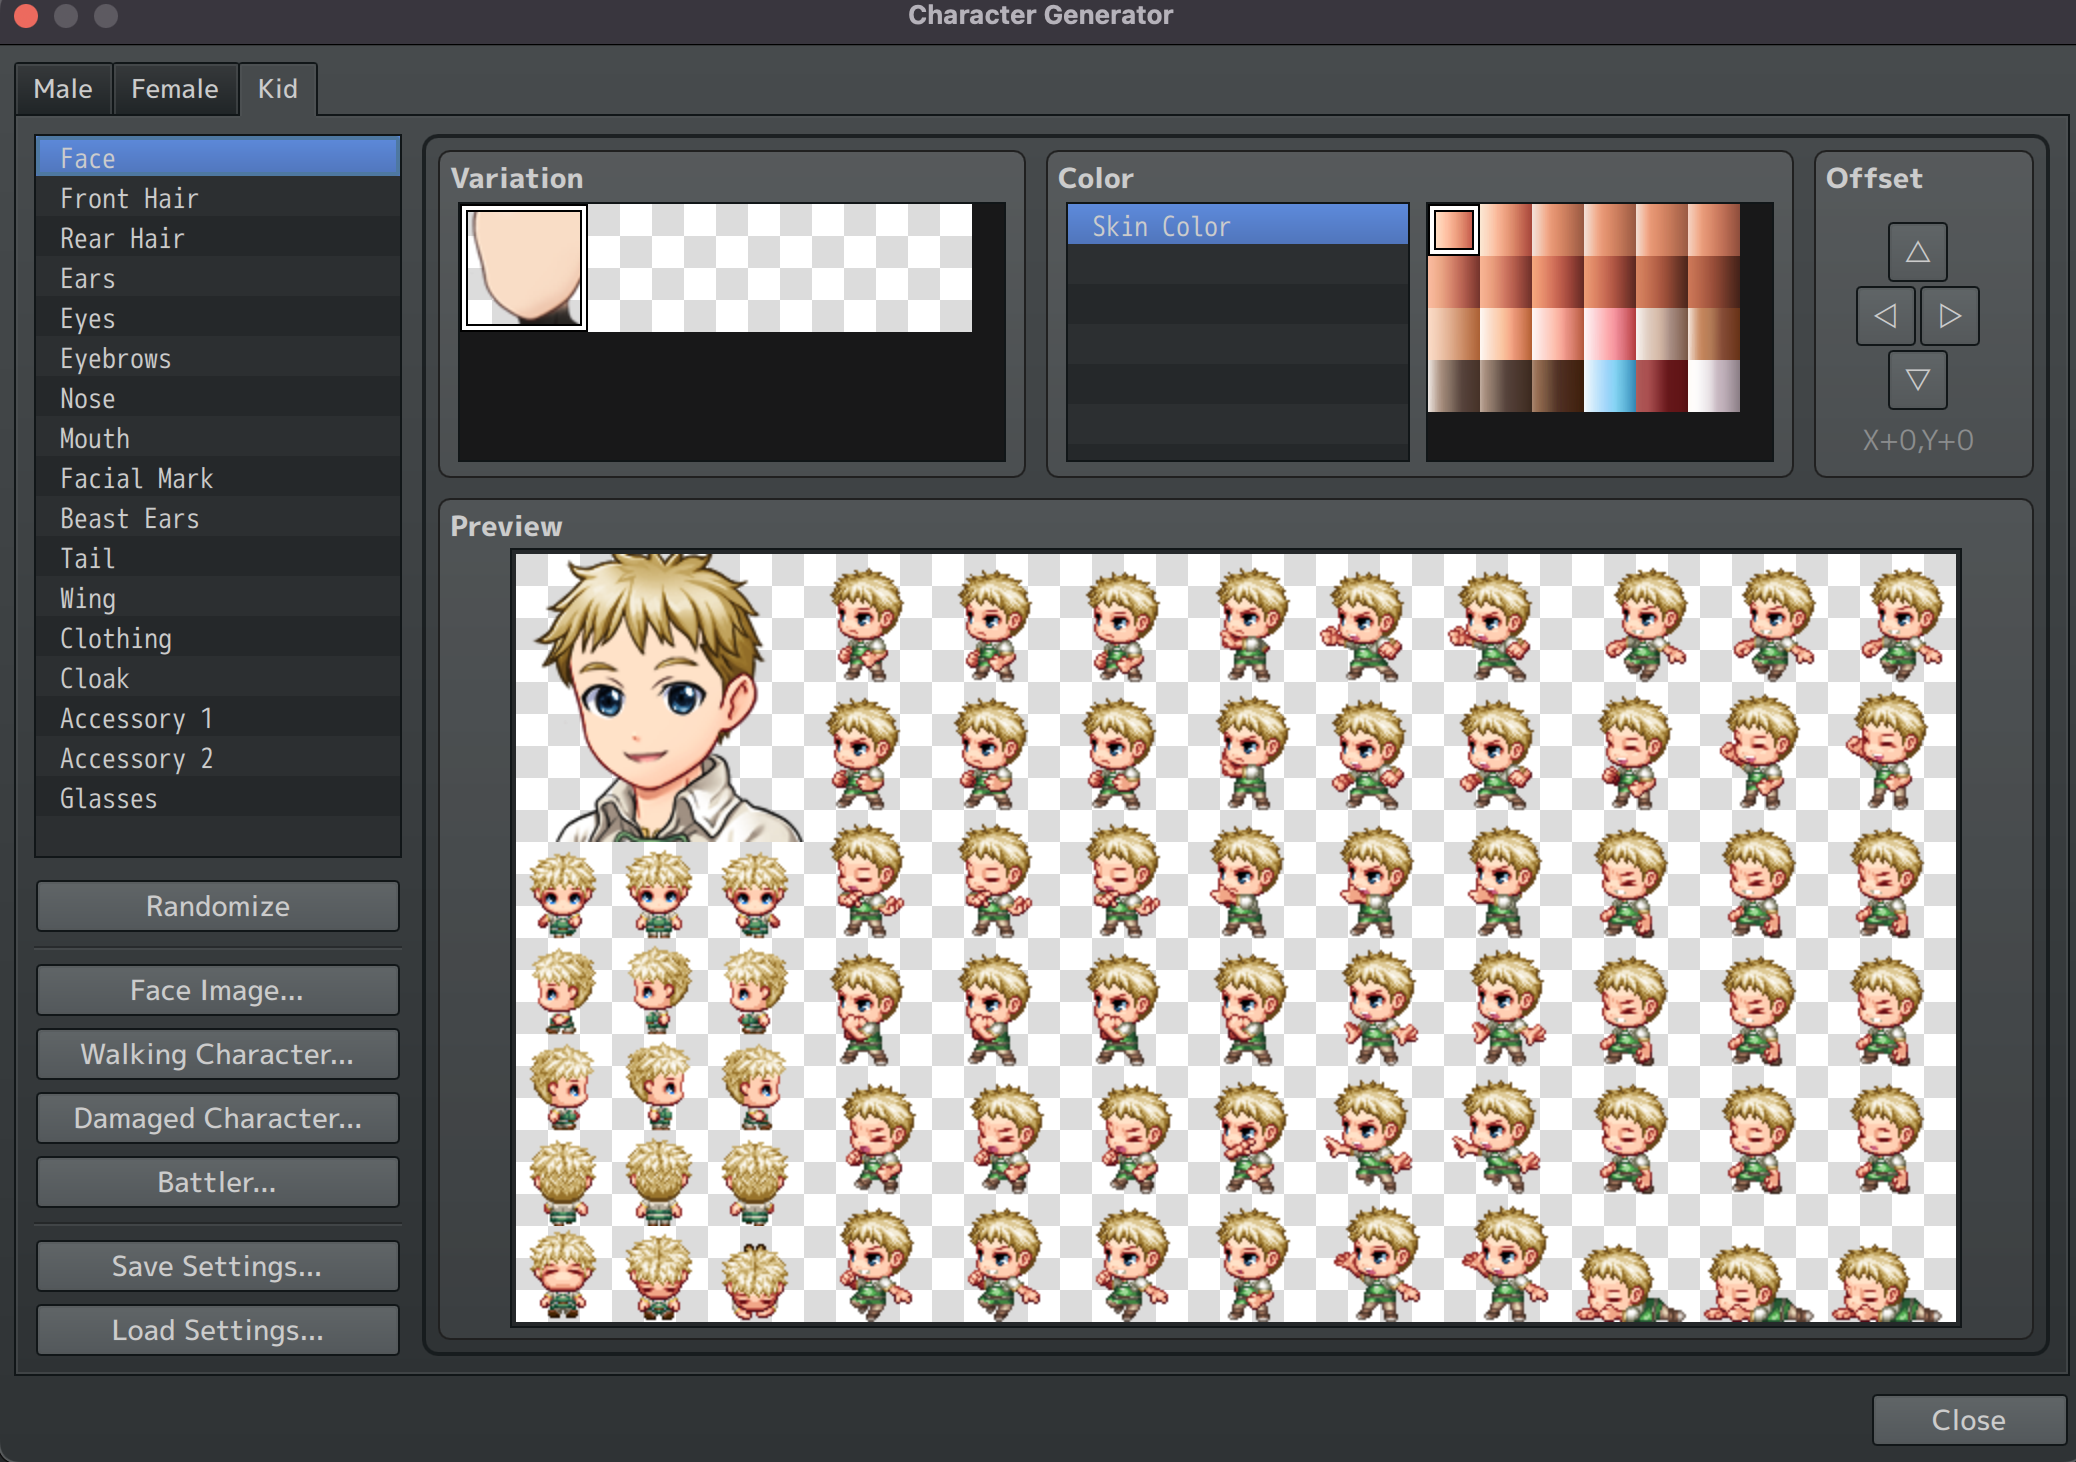
\includegraphics[scale=0.25]{Textuais/Pictures/Picture5.png}
	\fonte{Captura de tela do autor (2023).}\label{fig:rpgmaker-criador-personagens}
\end{figure}

\newpage

\subsubsection*{Banco de Dados}
O banco de dados incorporado ao RPG Maker MZ~\cite{RPGMakerMZ} é um componente central da plataforma, servindo como o núcleo para a gestão de diversos elementos essenciais à criação e ao desenvolvimento do jogo. Como ilustrado na Figura~\ref{fig:rpgmaker-interface-database}, o banco de dados permite o armazenamento e a manipulação de uma vasta gama de dados, incluindo:

\begin{itemize}
	\item \textbf{Actors}: Define os personagens jogáveis, incluindo seus nomes, classes, aparências e equipamentos iniciais. Cada ator pode ser detalhadamente customizado, contribuindo para a sua singularidade no universo do jogo.
	\item \textbf{Items}: Permite a criação e configuração de itens que podem ser utilizados pelos personagens, incluindo armas, armaduras, poções e artefatos especiais, cada um com suas propriedades e efeitos definidos.
	\item \textbf{Tilesets}: Conjuntos de tiles que são usados para construir os mapas do mundo do jogo, desde ambientes naturais a construções, proporcionando a base para a criação de cenários diversificados.
	\item \textbf{Common Events}: Eventos que podem ser chamados em diversas circunstâncias dentro do jogo, facilitando a reutilização de lógicas de eventos e a organização do fluxo de jogo.
	\item \textbf{System 1}: Configurações do sistema que incluem a música de fundo e os sons por padrão, as opções de batalha, e outras definições gerais que afetam o comportamento global do jogo.
	\item \textbf{System 2}: Continuação das configurações do sistema onde se podem ajustar os termos utilizados no jogo, os gráficos da janela de comando, entre outras opções que personalizam ainda mais a experiência do jogador.
\end{itemize}

\begin{figure}[ht]
	\centering
	\caption{Interface do Banco de dados do jogo no RPG Maker MZ~\cite{RPGMakerMZ}.}
	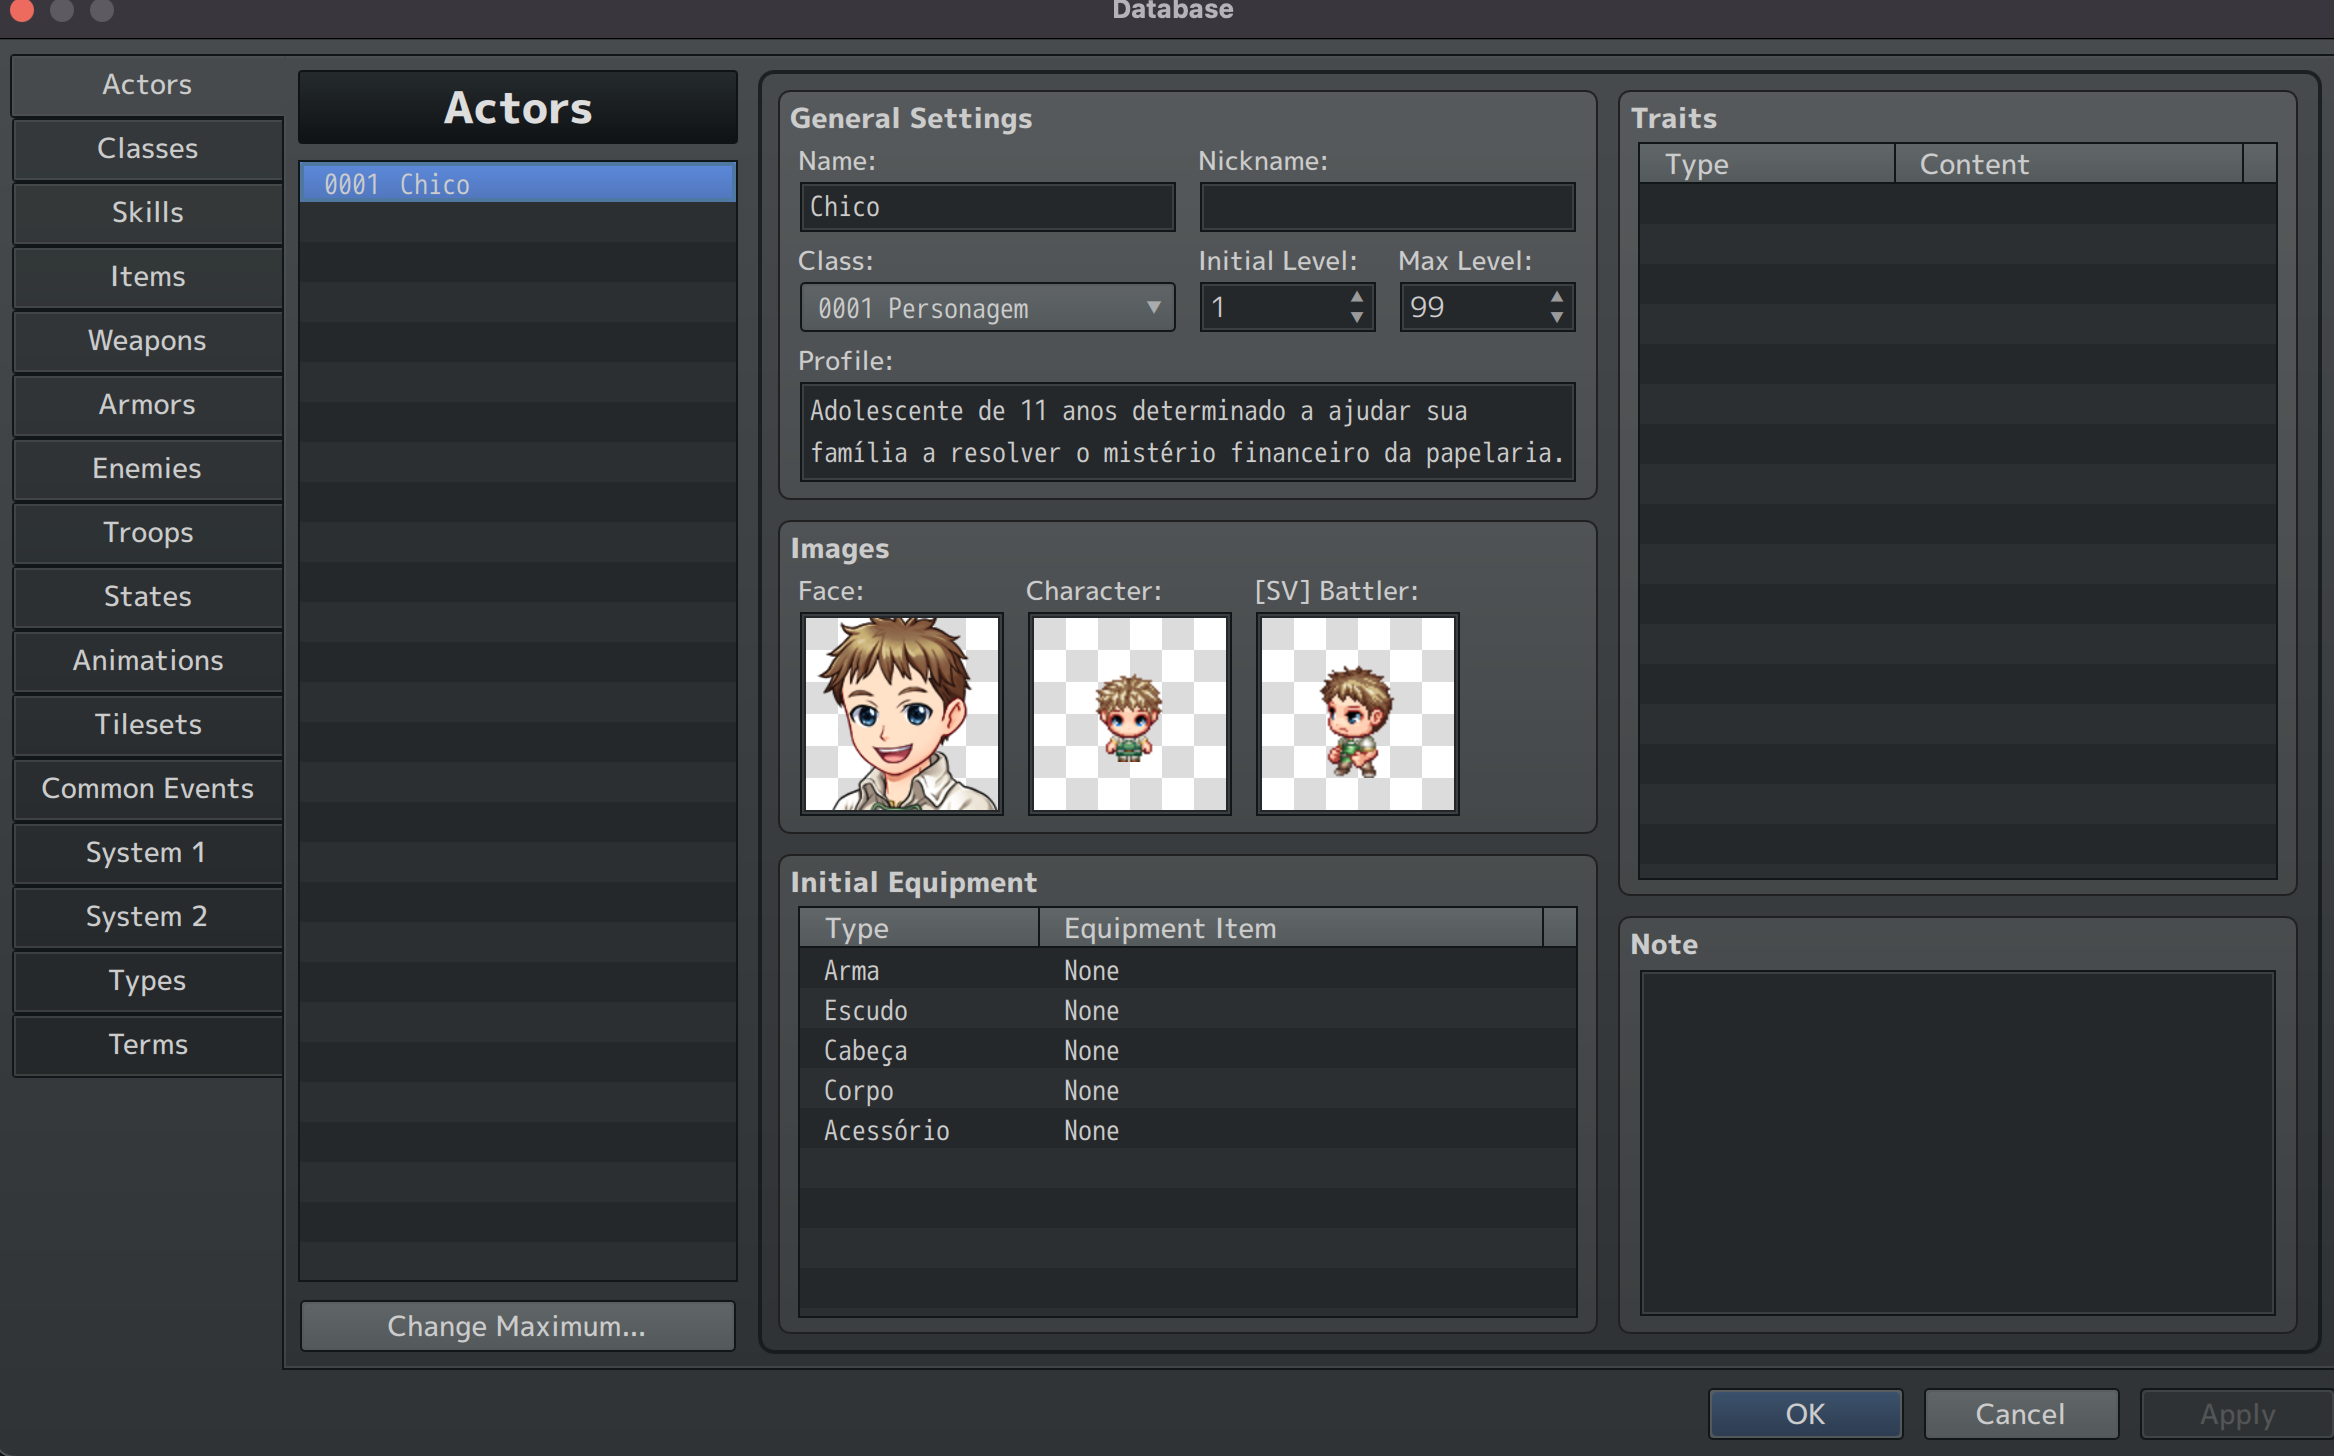
\includegraphics[scale=0.2]{Textuais/Pictures/DataBase.png}
	\fonte{Captura de tela do autor (2023).}\label{fig:rpgmaker-interface-database}
\end{figure}

\newpage

\section{GIMP}

O GIMP (\textit{GNU Image Manipulation Program}) é uma ferramenta de edição de imagens de código aberto, robusta e multiplataforma, que se revela uma escolha eficiente para a edição de \textit{tilesets} utilizados no RPG Maker MZ. Sua funcionalidade de manipulação de imagens permite aos desenvolvedores modificar e criar \textit{tilesets} personalizados, proporcionando um nível adicional de personalização e originalidade aos mapas do jogo. O GIMP suporta uma ampla gama de formatos de arquivo e oferece um leque de ferramentas de edição, desde simples cortes e ajustes de cores até operações complexas de manipulação de camadas e efeitos \cite{GIMP_Documentation}.

\begin{figure}[ht]
	\centering
	\caption{Interface de edição de imagem do \cite{GIMP_Documentation}.}
	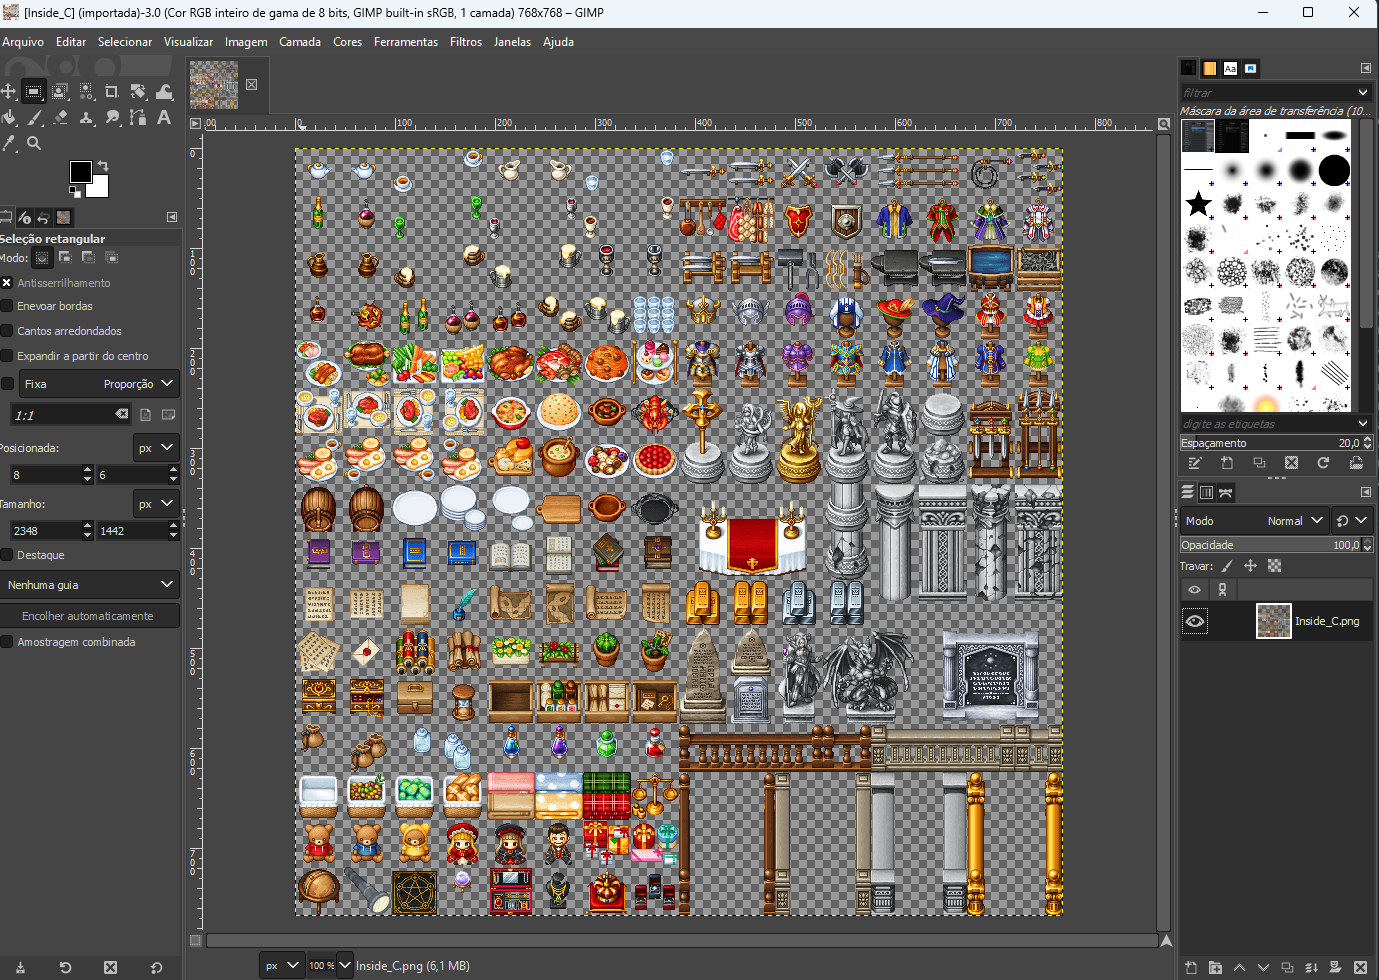
\includegraphics[scale=0.4]{Textuais/Pictures/Gimp.png}
	\fonte{Captura de tela do autor (2023).}\label{fig:gimp-interface}
\end{figure}

\section{Trabalhos Correlatos}
Esta seção apresenta alguns trabalhos que, de alguma forma, se correlacionam com o presente estudo, oferecendo uma perspectiva sobre as diversas abordagens em jogos educativos focados na educação financeira.

\subsection{Debt Maze}
O \textit{Debt Maze} \cite{Debt_Maze} representa um marco na integração de conceitos financeiros em jogos digitais. Esse jogo utiliza um labirinto repleto de desafios baseados em temas financeiros, como empréstimos, juros e pagamentos em atraso, criando uma experiência envolvente que se adapta a jogadores de diferentes níveis de conhecimento em finanças. A mecânica de navegação pelo labirinto simboliza as decisões financeiras na vida real, integrando elementos imersivos e persuasivos para educar e entreter o jogador. Essa abordagem lúdica contribui significativamente para a alfabetização financeira, incentivando decisões mais informadas.\com{É um jogo feito fora do Brasil? Se sim, pode comentar (no parágrafo abaixo) que seu jogo é focado no publico brasileiro, por seguir a ENEF e ser em português. Um jogo em inglês não é adequado para aplicação com estudantes brasileiros.}

Comparativamente, o presente trabalho distingue-se do \textit{Debt Maze} por adotar uma abordagem prática e cotidiana, mais adequada ao público infantil. Ao invés de um jogo de labirinto, propõe-se cenários reais e ferramentas interativas para simular decisões financeiras, aproximando o aprendizado à realidade das crianças. Além disso, por se basear na proposta da ENEF, o jogo desenvolvido neste trabalho é adequado para aplicação no ensino de educação financeira no Ensino Fundamental.

\icom{Mesmo comentário: as figuras precisam ser referenciadas e comentadas no texto (o que apresentam, etc).}

\icom{As duas figuras do Debt Maze têm o mesmo caption. Apresentar mais detalhes no caption, diferenciando as duas figuras, ou manter somente uma delas.}

\begin{figure}[ht]
	\centering
	\caption{Interface do Debt Maze.}
	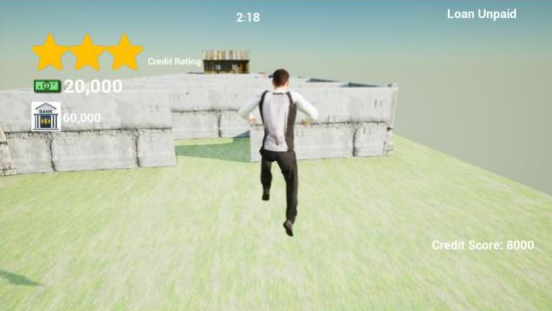
\includegraphics[scale=0.9]{Textuais/Pictures/debt-maze-1.png}
	\fonte{\textit{Debt Maze} \cite{Debt_Maze}.}\label{fig:debt-maze-1}
\end{figure}

\begin{figure}[ht]
	\centering
	\caption{Interface do Debt Maze.}
	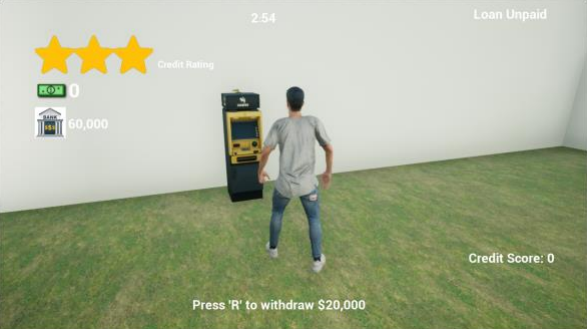
\includegraphics[scale=0.8]{Textuais/Pictures/debt-maze-2.png}
	\fonte{\textit{Debt Maze} \cite{Debt_Maze}.}\label{fig:debt-maze-2}
\end{figure}

\subsection{PlanCash}
O \textit{PlanCash} \cite{mariano2020educaccao}, um inovador jogo de tabuleiro, combina educação e entretenimento, utilizando a estrutura lúdica para ensinar matemática e gestão financeira a um público infantil. Este jogo aborda conceitos como a história do dinheiro e economia por meio de um tabuleiro interativo, onde os jogadores enfrentam situações-problema que estimulam a reflexão e análise financeiras. Essa abordagem didática destaca-se por integrar o aprendizado financeiro em atividades cotidianas, oferecendo uma base sólida para o entendimento infantil de conceitos financeiros e matemáticos.

Em contraste com esse jogo, o presente trabalho avança a ideia com uma proposta digital e atraente à geração atual de crianças, combinando elementos visuais e interativos para enriquecer a experiência educacional, alinhando o aprendizado financeiro às tecnologias contemporâneas.\com{Não está clara a diferença. Ambos são jogos digitais, certo? Então a diferença principal é o estilo RPG, que pode ser mais atrativo que um jogo digital no estilo de tabuleiro.}

\begin{figure}[ht]
	\centering
	\caption{Manual do \textit{PlanCash}.}
	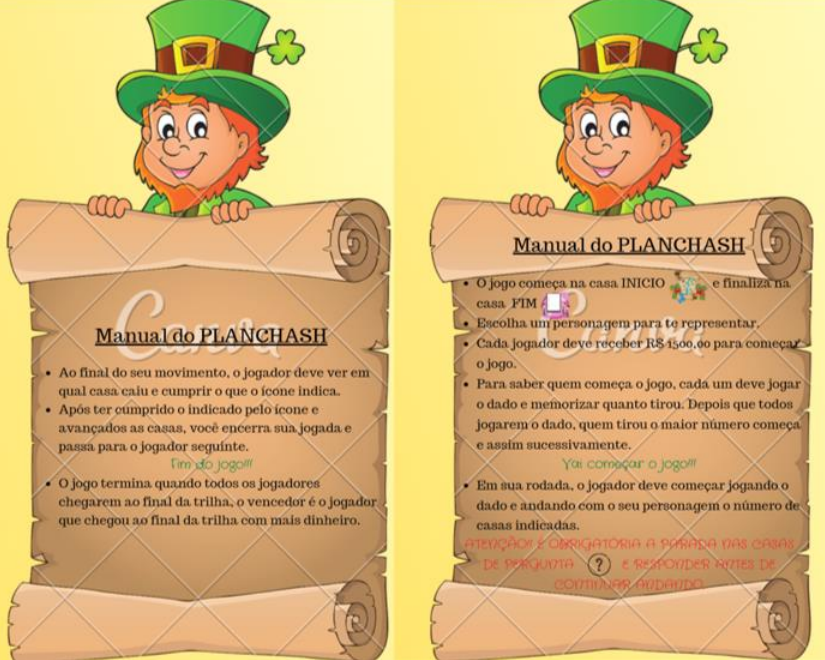
\includegraphics[scale=0.5]{Textuais/Pictures/Plancash-1.png}
	\fonte{\textit{PlanCash} \cite{mariano2020educaccao}.}\label{fig:plancash-1}
\end{figure}

\begin{figure}[ht]
	\centering
	\caption{Tabuleiro do \textit{PlanCash}.}
	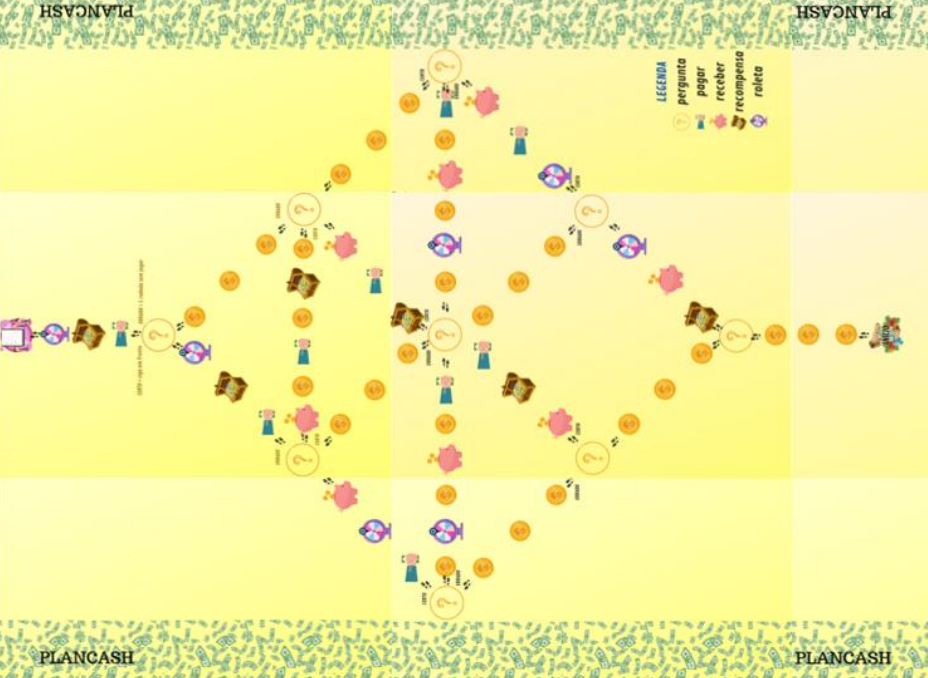
\includegraphics[scale=0.5]{Textuais/Pictures/Plancash-2.png}
	\fonte{\textit{PlanCash} \cite{mariano2020educaccao}.}\label{fig:plancash-2}
\end{figure}

\newpage

\subsection{Finance Game}

O \textit{Finance Game} \cite{Finance_Game} adota uma abordagem de simulação para a educação financeira, oferecendo aos jogadores cenários da vida adulta, como a gestão de um orçamento pessoal. Esse jogo destaca-se por seu foco na tomada de decisões financeiras equilibradas, promovendo um entendimento prático sobre responsabilidade financeira e bem-estar pessoal. A interação com elementos simulados do cotidiano, como mercado e banco, proporciona aos jogadores uma vivência educacional que transcende a mera teoria, enfatizando a importância de escolhas conscientes.

Em comparação, o presente trabalho foca em uma imersão mais alinhada à realidade infantil, oferecendo cenários e decisões financeiras que se conectam diretamente às experiências e compreensão das crianças, facilitando a assimilação dos conceitos de educação financeira.

\begin{figure}[ht]
	\centering
	\caption{Tela Inicial do \textit{Finance Game}.}
	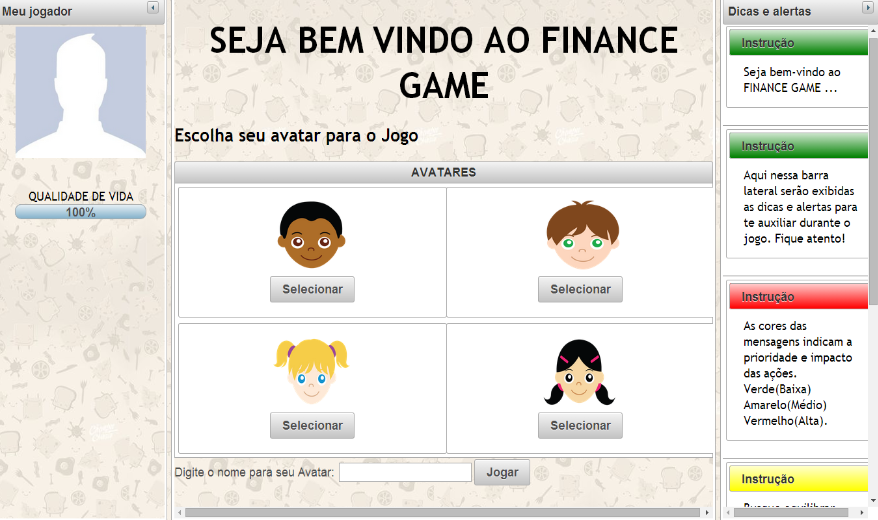
\includegraphics[scale=0.6]{Textuais/Pictures/Finance-game-1.png}
	\fonte{\textit{Finance Game} \cite{Finance_Game}.}\label{fig:finance-game-1}
\end{figure}

\begin{figure}[ht]
	\centering
	\caption{Cena do Mercado em \textit{Finance Game}.}
	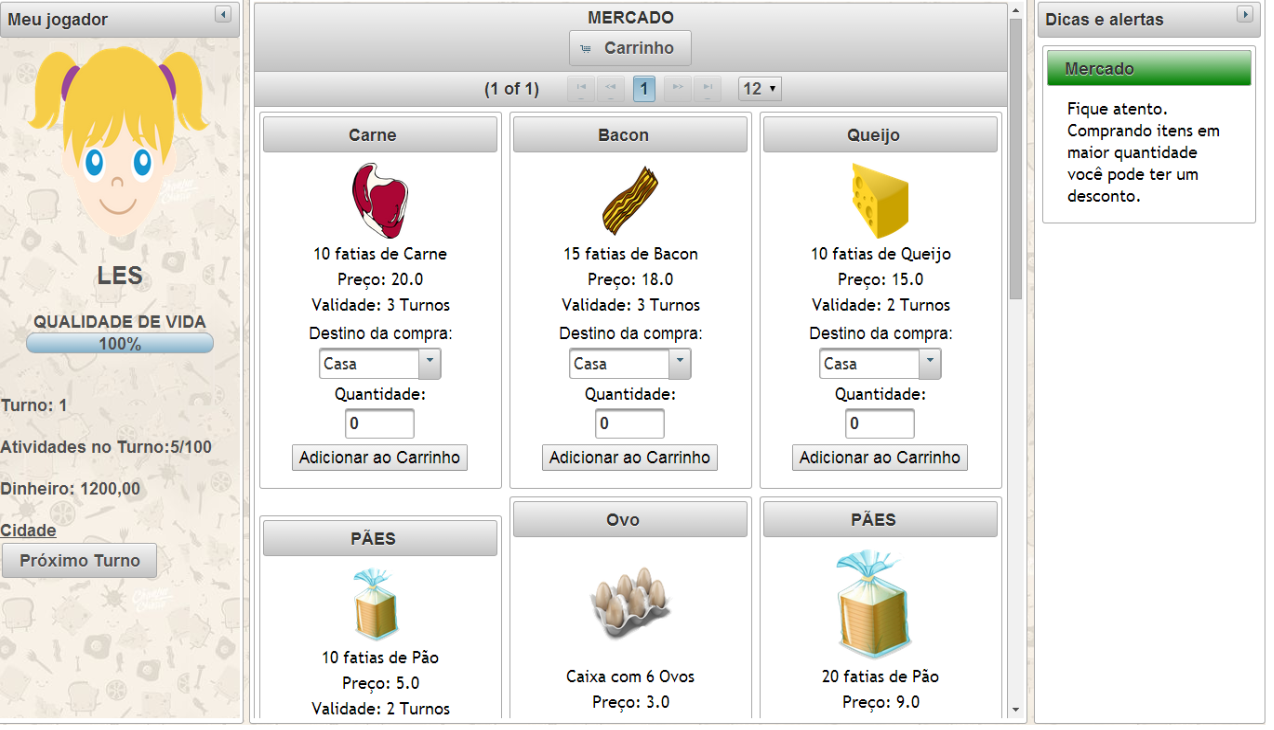
\includegraphics[scale=0.4]{Textuais/Pictures/Finance-game-2.png}
	\fonte{\textit{Finance Game} \cite{Finance_Game}.}\label{fig:finance-game-2}
\end{figure}

\newpage

\subsection{InvestPlay}
O \textit{InvestPlay} \cite{santos2020investplay} é um exemplo de jogo educativo que combina diversão e aprendizado em finanças. Esse jogo introduz os jogadores à gestão de ativos e passivos, adotando uma mecânica interativa de perguntas e respostas. O nível desafiador de algumas perguntas é uma consideração importante, especialmente para o público infantil. A personalização do jogo para diferentes temas educativos é um ponto forte, permitindo adaptar o conteúdo ao nível de compreensão das crianças.

Comparando-o com o presente estudo, busca-se refinar a proposta educacional do \textit{InvestPlay}, alinhando os conteúdos especificamente ao entendimento infantil. Esta abordagem simplificada visa tornar os conceitos financeiros mais acessíveis e relevantes para crianças, facilitando a assimilação eficaz dos princípios financeiros.\com{Além disso, um RPG é mais atrativo que um jogo de perguntas e respostas. Cabe pontuar essa diferença.}

\begin{figure}[ht]
	\centering
	\caption{Tela de instruções iniciais do \textit{InvestPlay}.}
	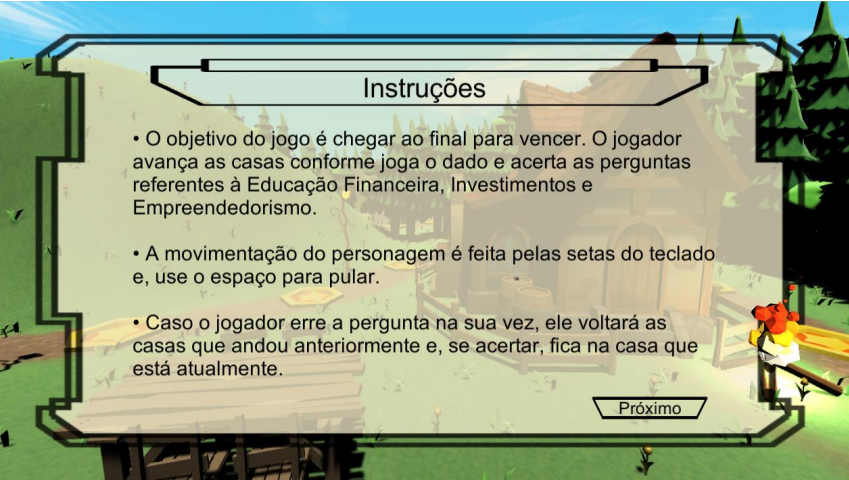
\includegraphics[scale=0.6]{Textuais/Pictures/invest-play-1.png}
	\fonte{\textit{InvestPlay} \cite{santos2020investplay}.}\label{fig:invest-play-1}
\end{figure}

\begin{figure}[ht]
	\centering
	\caption{Cena do jogo \textit{InvestPlay}.}
	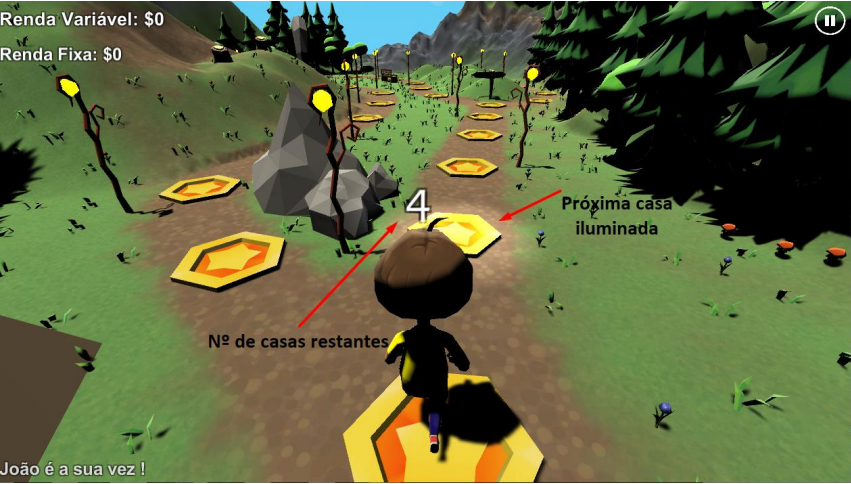
\includegraphics[scale=0.6]{Textuais/Pictures/invest-play-2.png}
	\fonte{\textit{InvestPlay} \cite{santos2020investplay}.}\label{fig:invest-play-2}
\end{figure}

\subsection{Considerações sobre os Trabalhos Correlatos}
Esta seção evidencia a diversidade de abordagens em jogos educativos focados em finanças, cada um com suas características distintas. A gamificação, como demonstrado nos exemplos citados, é uma ferramenta eficaz para a educação financeira, adaptando-se a diferentes públicos e objetivos de aprendizagem. No entanto, ressalta-se a importância de alinhar a metodologia e o conteúdo ao público-alvo, especialmente ao lidar com conceitos financeiros para crianças, onde a simplicidade e a relevância dos conteúdos são fundamentais.

\icom{Referenciar e comentar a tabela no texto.}

\begin{table}[ht]
	\centering
	\renewcommand{\arraystretch}{1.3}
	\caption{Comparativo Aprofundado dos Trabalhos Correlatos}
	\label{tab:comparativo-trabalhos}
	\begin{tabular}{| L{2.5cm} | L{2.6cm} | L{2.6cm} | L{2.6cm} | L{2.6cm} | L{2.6cm} |}
		\hline
		\textbf{}                       & \textbf{Debt Maze}       & \textbf{PlanCash}                    & \textbf{Finance Game}        & \textbf{InvestPlay}               \\
		\hline
		\hline
		\textbf{Público-Alvo}           & Geral                    & Infantil                             & Geral                        & Geral                             \\
		\hline
		\textbf{Metodologia}            & Labirinto                & Jogo de Tabuleiro                    & Simulação                    & Perguntas e Respostas             \\
		\hline
		\textbf{Abordagem Pedagógica}   & Gamificação              & Gamificação e Educação Tradicional   & Simulação Realista           & Dinâmica Interativa               \\
		\hline
		\textbf{Integração Tecnológica} & Média                    & Baixa                                & Média                        & Média                             \\
		\hline
		\textbf{Impacto Educacional}    & Alfabetização Financeira & Conhecimento Financeiro e Matemático & Tomada de Decisão Financeira & Entendimento de Ativos e Passivos \\
		\hline
		\textbf{Baseado na ENEF}        & Não                      & Não                                  & Não                          & Não                               \\
		\hline
	\end{tabular}
	\vspace{2mm}
	\fonte{Elaborado pelo autor (2023).}
\end{table}
